\documentclass[10pt]{beamer}

\usetheme{metropolis}
\usecolortheme{beaver}
\usepackage{appendixnumberbeamer}

\usepackage{booktabs}
\usepackage[scale=2]{ccicons}

\usepackage{pgfplots}
\usepgfplotslibrary{dateplot}

\usepackage{xspace}
\newcommand{\themename}{\textbf{\textsc{metropolis}}\xspace}
%\usepackage[brazil]{babel}  % AAB
\usepackage{bibentry}       % AAB
\usepackage{amsmath, bm}    % AAB
\usepackage{tikz}           % AAB    
\usetikzlibrary{shapes,arrows,shadows}  % AAB inserido
%\usepackage[utf8]{inputenc}                  % AAB inserido
                                              % AAB inserido
\usepackage[caption=false,font=normalsize,labelfont=sf,textfont=sf]{subfig}
%\usepackage[caption=false,font=footnotesize]{subfig}
%
\DeclareMathOperator{\traco}{tr} %AAB
\graphicspath{{../Dissertacao/figuras/}}        % AAB - caminho das figuras
%\graphicspath{{../Images/PDF/}}                 % AAB - caminho das figuras (recomendável) 

\title{Fusion of Evidences for Edge Detection in PolSAR Images}
%\subtitle{A modern beamer theme}
\date{\today}
\author{Anderson Adaime de Borba - Mackenzie-BR - IBMEC-SP\\
        Dr. Mauricio Marengoni - Mackenzie-BR\\
        Dr. Alejandro Frery - UFAL-BR} 
\institute{TENGARSS- 2019}
\titlegraphic{\hfill
\includegraphics[height=1.1cm]{logo_mack1.pdf}}
\titlegraphic{\hfill
\includegraphics[height=1.1cm]{laccan_ufal.pdf}}

\titlegraphic{%
      
\includegraphics[width=.2\textwidth]{laccan_ufal.pdf}\hfill
     % 
\includegraphics[width=3cm,height=1.6cm]{ufal.pdf}\hfill
      
\includegraphics[width=.2\textwidth]{logo_mack1.pdf}
   }

\begin{document}

\maketitle

%\begin{frame}{Schedule}
%  \setbeamertemplate{section in toc}[sections numbered]
%  \tableofcontents[hideallsubsections]
%\end{frame}

\begin{frame}[fragile]{PolSAR Image}
\begin{alertblock}{PolSAR important characteristics}
\begin{itemize}
%\item[-] can be on raised platforms, crewed aircraft or not, satellites orbiting the  earth or other planets;
%\item[-] it is a viable and practical imaging technique;
\item[-] PolSAR images has a high resolution;
%\item[-] synthesizes long antenna openings;
\item[-] radars produce images day and night;
\item[-] climate does not interfere in image capture;
%\item[-] SAR imaging systems operate in the microwave region of the electromagnetic spectrum, usually between the P-band - and the K-band.
\end{itemize}
\end{alertblock}
\begin{alertblock}{PolSAR Applications}
\begin{itemize}
\item[-] Remote sensing;
\item[-] economy;
\item[-] topography;
\item[-] oceanography;
%\item[-] glaciology;
\item[-] agriculture
%\item[-] geology;
\item[-] forests;
\item[-] fixed or moving targets;
\item[-] environmental monitoring;
%\item[-] oil spill control;
%\item[-] moreover, the aid of optical systems.
\end{itemize}
\end{alertblock}
\end{frame}

%\begin{frame}[fragile]{PolSAR Image}
%\begin{alertblock}{PolSAR Applications}
%\begin{itemize}
%\item[-] Remote sensing;
%\item[-] economy
%\item[-] topography;
%\item[-] oceanography;
%\item[-] glaciology;
%\item[-] agriculture
%\item[-] geology;
%\item[-] forests;
%\item[-] fixed or moving targets;
%\item[-] environmental monitoring;
%\item[-] oil spill control;
%\item[-] moreover, the aid of optical systems.
%\end{itemize}
%\end{alertblock}
%\end{frame}

\begin{frame}[fragile]{PolSAR Image}
\begin{alertblock}{Statistical modeling for PolSAR data (1 - Look)}
\begin{itemize}
\item The complex scattering matrix $\mathbf{S}$:
\begin{equation}
\mathbf{S} = \left[
\begin{array}{cc}
	S_\text{hh}   & S_\text{hv}   \\
	S_\text{vv}   & S_\text{vv}   
\end{array}
\right].
\end{equation}\label{eq_01}
\item The medium of propagation of waves is reciprocal
$$\mathbf{s}=[S_\text{hh},S_\text{hv},S_{\text{vv}}]^T.$$
\end{itemize}
\end{alertblock}
\end{frame}

\begin{frame}[fragile]{PolSAR Image}
\begin{alertblock}{Statistical modeling for PolSAR data (1 - Look)}
\begin{itemize}
\item The probability density function (pdf):
\begin{equation}
    f_{\mathbf{s}}(\mathbf{s};\Sigma)=\frac{1}{\pi^3|\Sigma|} \exp(-\mathbf{s}^H\Sigma^{-1}\mathbf{s}),
    \label{eq_02}
\end{equation}
        \begin{description}
        \item[-] $|\cdot|$ is the determinant, 
        \item[-] $H$ denotes the conjugate complex number, 
        \item[-] $\Sigma$ is the covariance matrix of $\mathbf{s}$ such that $\Sigma=E[\mathbf{ss}^H]$,
        \item[-] $E[\cdot]$ denotes the expected value. 
        \item[-] The distribution of $\mathbf{s}$ is assumed to be  Gaussian circular complex multivariate with zero mean $N^{C}_3(0,\Sigma)$.
        \end{description}
\end{itemize}
\end{alertblock}
\end{frame}
%
\begin{frame}[fragile]{PolSAR Image}
\begin{alertblock}{Statistical modeling for PolSAR data (L - Looks)}
\begin{itemize}
\item The estimated sample covariance matrix:
\begin{equation}
    \mathbf{Z}=\frac{1}{L}\sum_{\ell=1}^{L} {\mathbf{s}_\ell}{\mathbf{s}_\ell}^H,
    \label{eq_03}
\end{equation}
\begin{description}
      \item[-] $\mathbf{s}_\ell$, $\ell = 1, \dots, L$;
      \item[-] $L$ independent samples of complex vectors distributed as $\mathbf{s}$. 
\end{description}
\end{itemize}
\end{alertblock}
\end{frame}

\begin{frame}[fragile]{PolSAR Image}
\begin{alertblock}{Statistical modeling for PolSAR data (L - Looks)}
\begin{itemize}
\item Multilooked Wishart distribution with probability density function:
\begin{equation}
    f_{\mathbf{Z}}(\mathbf{Z};\Sigma_{s},L)=\frac{L^{mL}|\mathbf{Z}|^{L-m}}{|\Sigma_{s}|^{L}\Gamma_m(L)} \exp(-L\traco(\Sigma_{s}^{-1}\mathbf{Z})),
    \label{eq_04}
\end{equation} 
\begin{description}
\item[-] $\traco(\cdot)$ is the trace operator,
\item[-] $\Gamma_m(L)$ is a multivariate Gamma function
\begin{equation*}
	\Gamma_m(L)=\pi^{\frac{1}{2}m(m-1)} \prod_{i=0}^{m-1}\Gamma(L-i),
\end{equation*}
\item[-]$\Gamma(\cdot)$ is the Gamma function,
\item[-]$m=3$,
\item[-]$\mathbf{Z}\sim W(\Sigma, L)$, 
%\item[-]$E[\mathbf{Z}]=\Sigma$. 
\end{description} 
\end{itemize}
\end{alertblock}
\end{frame}

\begin{frame}[fragile]{PolSAR Image}
\begin{alertblock}{Edges detection}
The following procedure is proposed to detected edges in the $\text{hh}$, $\text{hv}$ and $\text{vv}$ channels:
\begin{itemize}
	\item identify the centroid of a region of interest (ROI) in an automatic, semi-automatic or manual manner;
	\item cast rays from the centroid to the outside of the area;
	\item collect data around the rays using the  Bresenham's midpoint line algorithm, ideally the size of a pixel;
	\item detect points in the data strips which provide evidence of changes in their statistical properties, i.e., a transition point that defines edge evidence;
	\item use the Generalized Simulated Annealing (GenSA) method, Ref.~\cite{xgsh}, to find maximum points in the functions of interest;
	\item fuse the evidence of detected edges in the $\text{hh}$, $\text{hv}$ and $\text{vv}$ channels.
\end{itemize}
\end{alertblock}
\end{frame}

\begin{frame}[fragile]{PolSAR Image}
\begin{alertblock}{Edges detection - ROI Flevoland Example} 
\begin{figure}[hbt]
\centering
	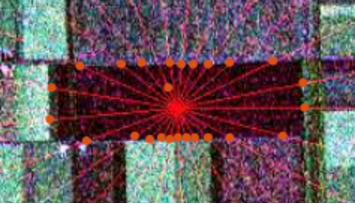
\includegraphics[width=.7\linewidth]{flevoland_radial_25_point_hh_crop}
	\caption{Edges detection example ($\text{hh}$ channel).}
\label{flevoland_radial_4look}
\end{figure}
\end{alertblock}
\end{frame}

%\begin{frame}[fragile]{PolSAR Image}
%\begin{alertblock}{Maximum Likelihood Estimator (MLE)}
%\begin{itemize}
%	\item Suppose $\mathbf{X}=(X_1,X_2,\dots,X_n)^T$ is a random vector distributed according to the probability density function $f(\mathbf{x},\mathbf{\theta})$ with parameters $\mathbf{\theta}=(\theta_1,\dots,\theta_d)^T$ in the parameter space $\Theta$.
%%    \item The likelihood function is
%%\begin{equation*}
%%    L(\theta;\mathbf{X}) = \prod_{i=1}^{n}f(x_i;\theta),
%%\end{equation*}
%    \item log-likelihood function is
%\begin{equation}
%	\ell(\theta;\mathbf{X})= \ln L(\theta;\mathbf{X}) = \sum_{i=1}^{n}\ln f(x_i;\theta),
%	\label{eq_05}
%\end{equation}
%     %\item $\widehat{\theta}= \arg\max\limits_{\theta\in\Theta}L(\theta;\mathbf{x})$,
%     \item $\widehat{\theta}= \arg\max\limits_{\theta\in\Theta}\ell(\theta;\mathbf{x})$.
%\end{itemize}
%\end{alertblock}
%\end{frame}

\begin{frame}[fragile]{PolSAR Image}
\begin{alertblock}{Maximum Likelihood Estimator (MLE) for two regions A and B}
\begin{itemize}
\item The estimates for the covariance matrices can be found using the maximum likelihood estimator denoted by $\widehat{\Sigma}$, Ref.~\cite{good}: 
\begin{equation}
\widehat{\Sigma_{I}}(j) = \left\{
\begin{array}{lc}
	j^{-1}\sum_{k=1}^{j}\mathbf{Z}_{k}  & \mbox{if}\quad I=A,  \\
        (N-j)^{-1}\sum_{k=j+1}^{N}\mathbf{Z}_{k} & \mbox{if}\quad I=B.
\end{array}
\right.\label{eq_08}
\end{equation}
%	\item likely function
%	 \begin{equation}
%	L(j)=\prod_{k_1=1}^{j}f_{\mathbf{Z}}(\mathbf{Z}_{k_1};\widehat\Sigma_{A},L) \prod_{k_2=j+1}^{N}f_{\mathbf{Z}}(\mathbf{Z}_{k_2};\widehat\Sigma_{B},L),
%	\label{eq_06}
%\end{equation}
    \item log-likely function
\begin{equation}
\ell(j) =
	\sum_{k_1=1}^{j}\ln f_{\mathbf{Z}}(\mathbf{Z}_{k_1}; \widehat\Sigma_{A},L) + \sum_{k_2=j+1}^{N}\ln f_{\mathbf{Z}}(\mathbf{Z}_{k_2}; \widehat\Sigma_{B},L).
	\label{eq_07}
\end{equation}
\end{itemize}
\end{alertblock}
\end{frame}


\begin{frame}[fragile]{PolSAR Image}
\begin{alertblock}{Maximum Likelihood Estimator (MLE)}
\begin{itemize}
	\item After algebraic manipulations on each term of the summation, it is obtained:
\begin{align}\nonumber
	\ell(j)&=N\left[mL(\ln{L}-1)-\ln{\Gamma_m(L)}\right]\\\nonumber
	&- L\left[j\ln{|\widehat{\Sigma}_{A}(j)|} +(N-j)\ln{|\widehat{\Sigma}_{B}(j)|}\right] \\
	&+ (L-m)\sum_{k=1}^{N}\ln{|\mathbf{Z}_{k}|}.\label{eq_09}
\end{align}

\item The argument of the maximum $\widehat{\jmath}$ is the edge evidence that will be used in our fusion methods.
\end{itemize}
\end{alertblock}
\end{frame}

\begin{frame}[fragile]{PolSAR Image}
\begin{alertblock}{Application in simulated images}
	\begin{figure}[hbt]
     \subfloat[Pauli decomposition \label{fig_Edges-Evidence:a}]{%
       %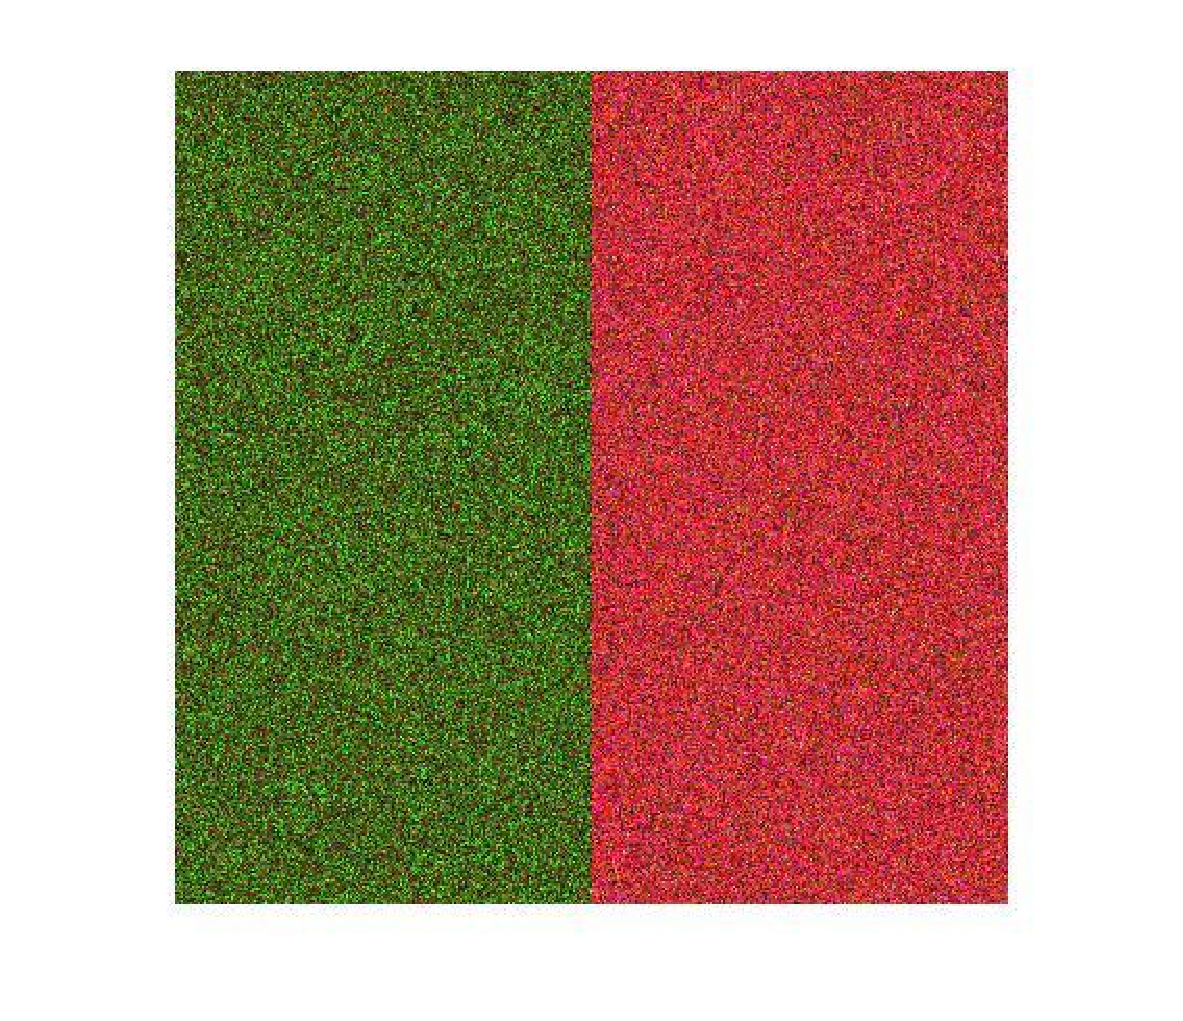
\includegraphics[viewport= 80 50 490 460, clip=true, width=0.23\textwidth]{phanton_nhfc_dec_pauli}}      
       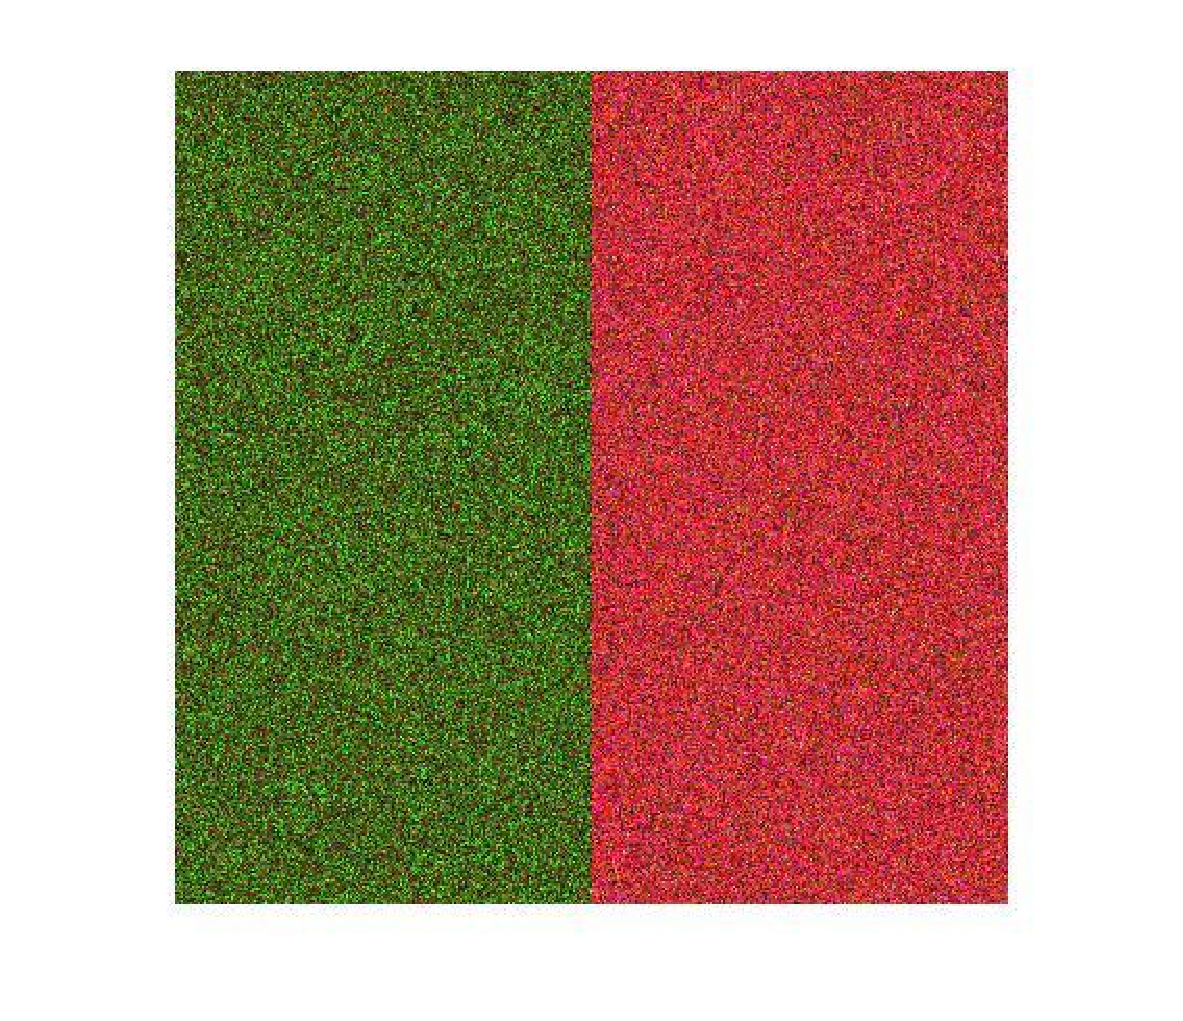
\includegraphics[viewport= 80 50 490 460, clip=true, width=0.35\textwidth]{phanton_nhfc_dec_pauli}}  
     \subfloat[Marginal densities of the $\text{hh}$ channel\label{fig_Edges-Evidence:b}]{%
       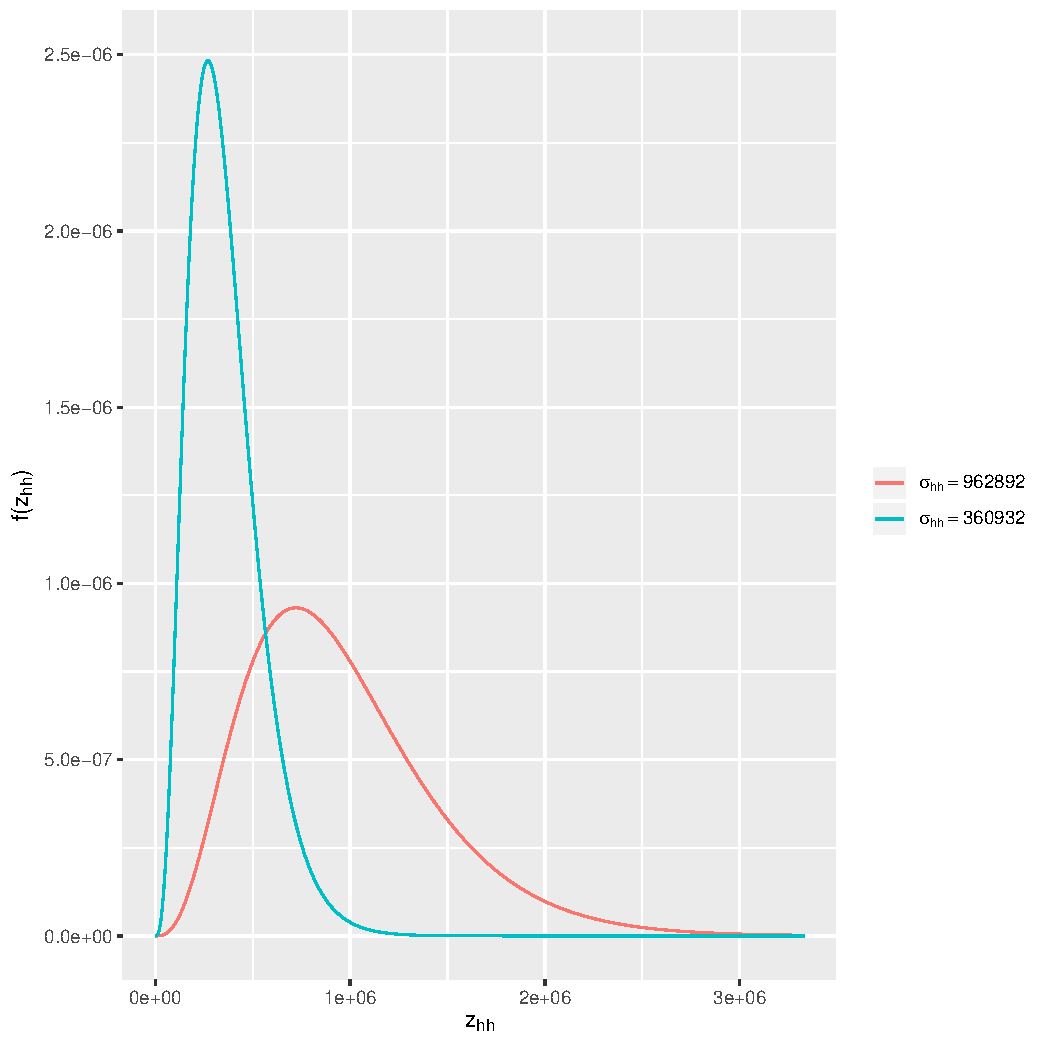
\includegraphics[width=0.34\textwidth]{grafico_pdf_nhfc_2014_sigma_hh_artigos}
     }
    %\caption{Edges evidences}
     \label{fig_Edges-Evidence}
\end{figure}
\end{alertblock}
\end{frame}



\begin{frame}[fragile]{PolSAR Image}
\begin{alertblock}{Application in simulated images}
	\begin{figure}[hbt]
	\centering
     \subfloat[Channel $\text{hh}$ \label{fig_evid_bordas:1a}]{%
       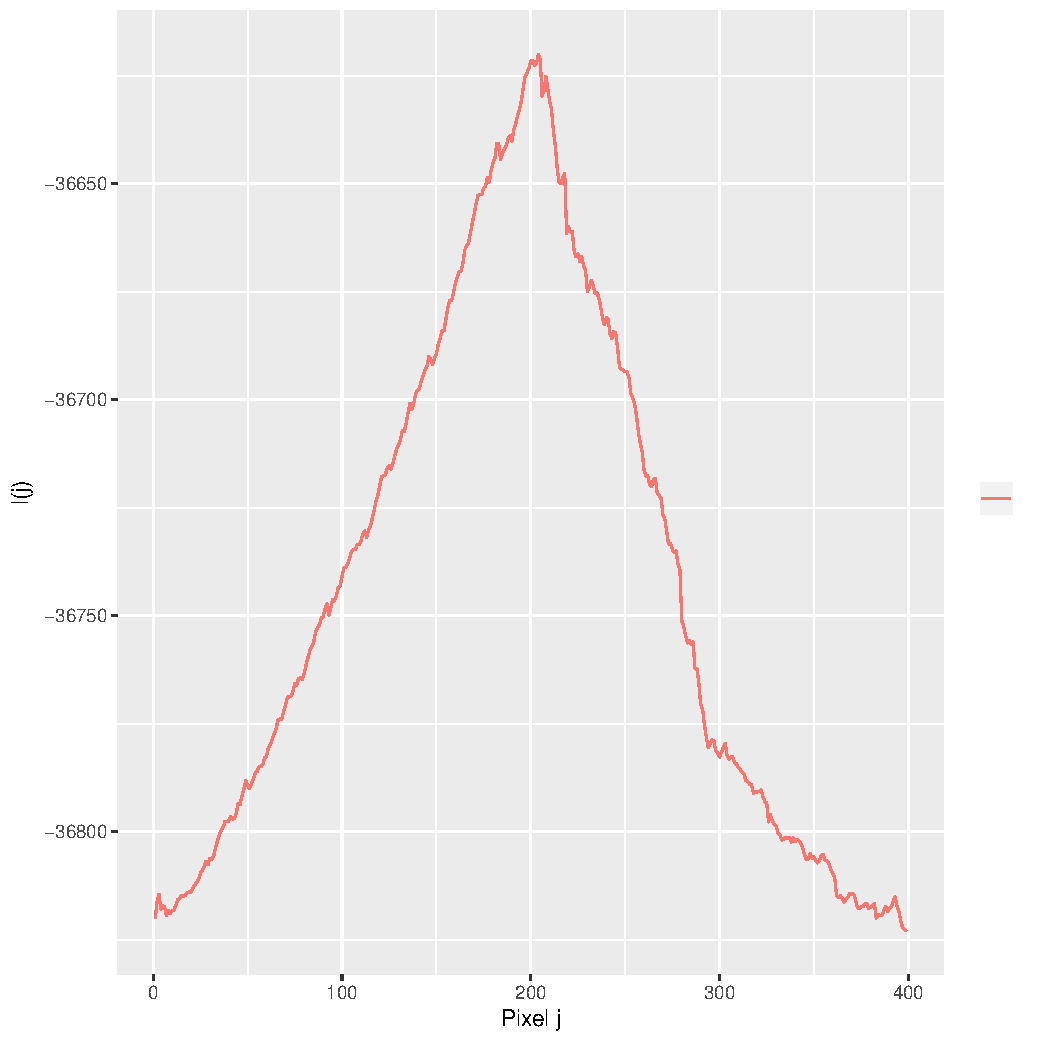
\includegraphics[width=0.32\linewidth]{grafico_l_nhfc_2014_sigmahh_artigos}}
     \subfloat[Channel $\text{hv}$ \label{fig_evid_bordas:1b}]{%
       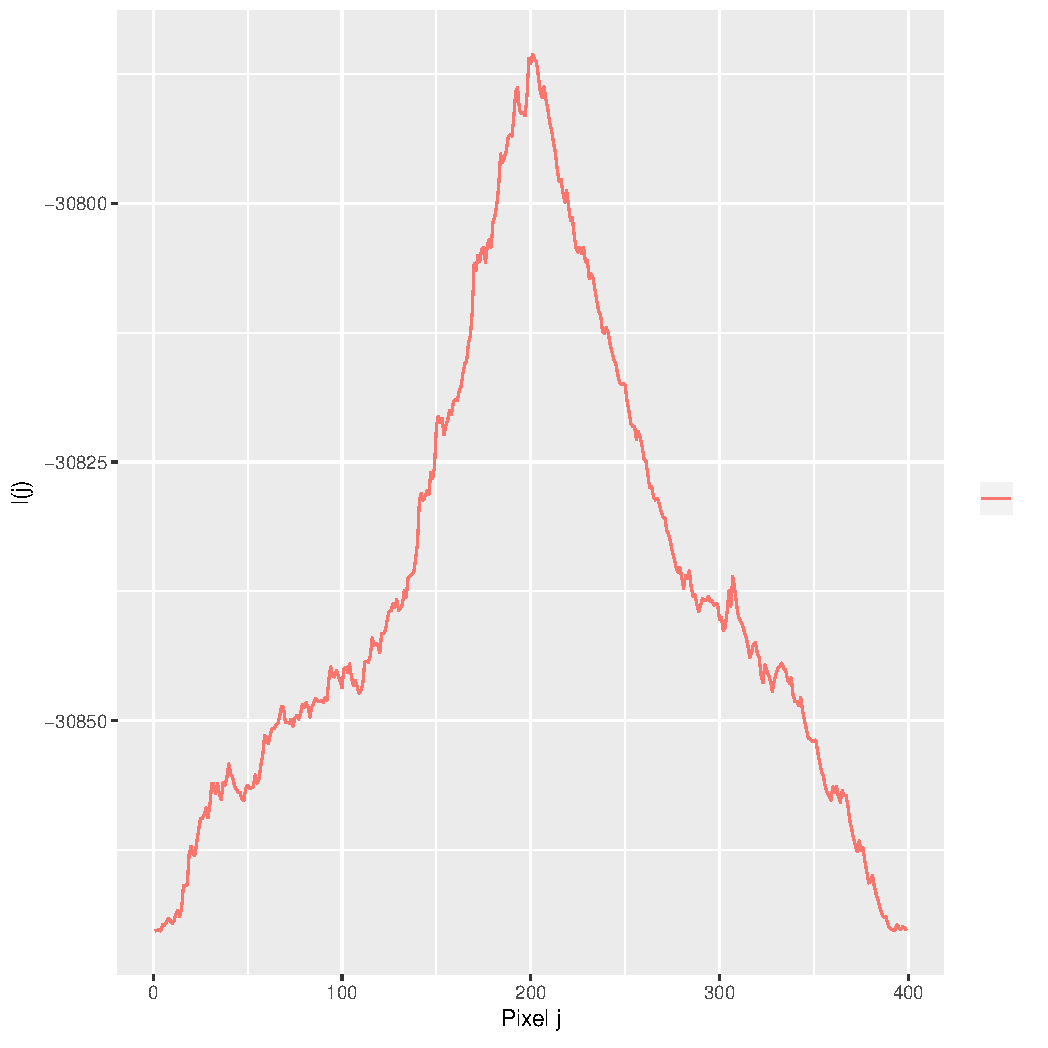
\includegraphics[width=0.32\linewidth]{grafico_l_nhfc_2014_sigmahv_artigos}}
     \subfloat[Channel $\text{vv}$ \label{fig_evid_bordas:1c}]{%
       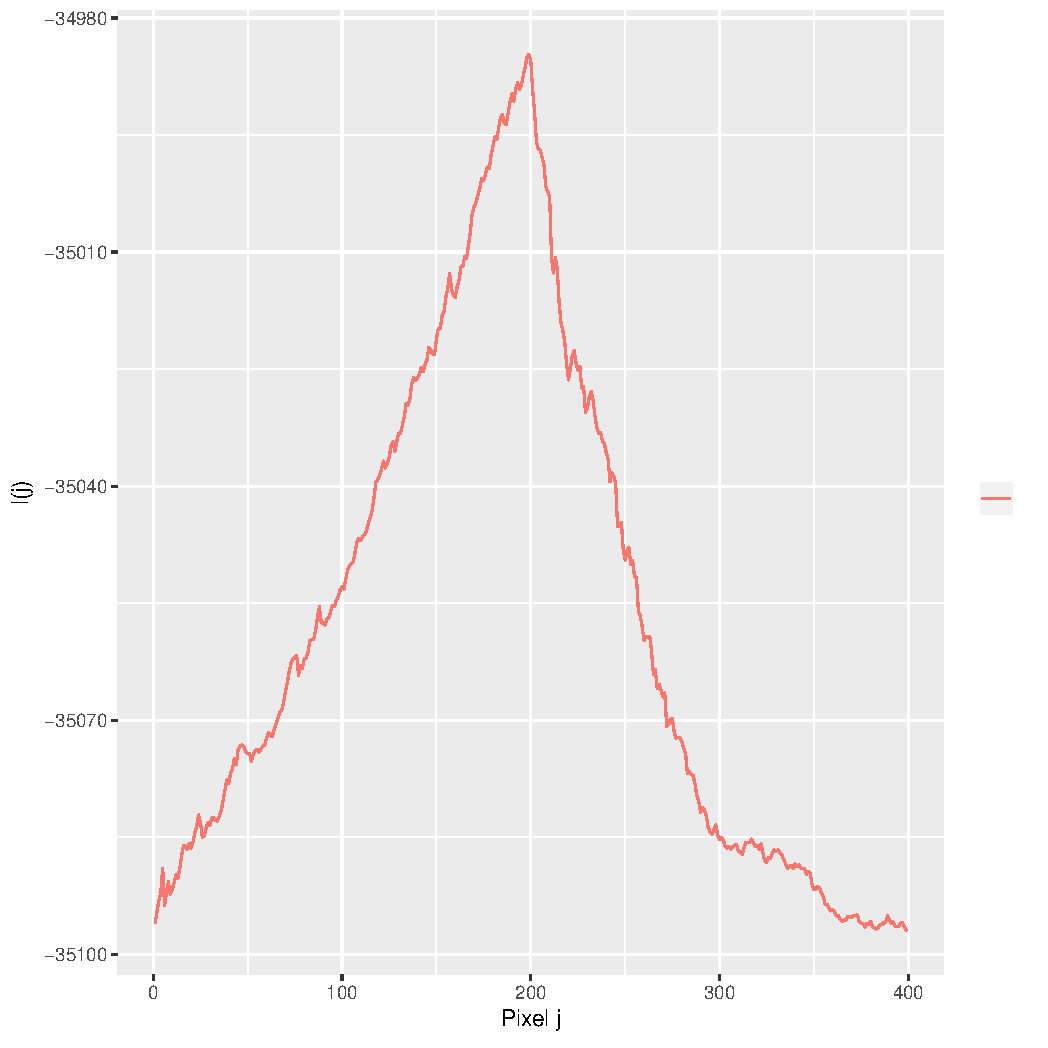
\includegraphics[width=0.32\linewidth]{grafico_l_nhfc_2014_sigmavv_artigos}}
     \caption{Edges evidences}
     \label{fig_evid_bordas}
   \end{figure}	
\end{alertblock}
\end{frame}


\begin{frame}[fragile]{PolSAR Image}
\begin{alertblock}{Application in simulated images} 
	\begin{figure}[hbt]
	\centering
	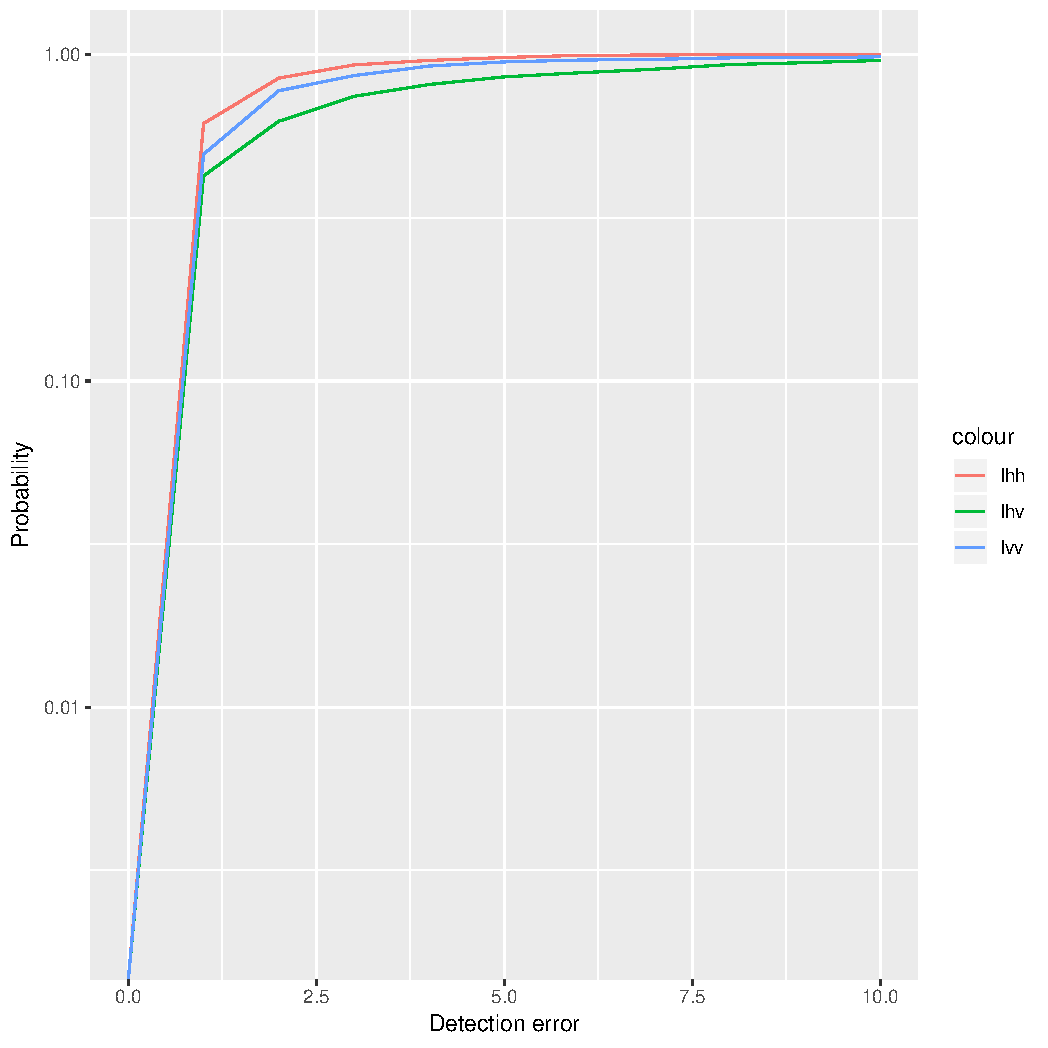
\includegraphics[width=.5\linewidth]{metricas_ihh_ivh_ivv_nhfc_artigos}%
	\caption{Probability of detecting edges evidences.}
\label{probability_edge_detc}
\end{figure}
\end{alertblock}
\end{frame}

\begin{frame}[fragile]{PolSAR Image}
\begin{alertblock}{Average Fusion}
\pgfdeclarelayer{background}
\pgfdeclarelayer{foreground}
\pgfsetlayers{background,main,foreground}
%
\pgfdeclarelayer{background}
\pgfdeclarelayer{foreground}
\pgfsetlayers{background,main,foreground}
\tikzstyle{sensor}=[draw, fill=blue!20, text width=5em, 
    text centered, minimum height=2.5em,drop shadow]
\tikzstyle{ann} = [above, text width=5em, text centered]
\tikzstyle{wa} = [sensor, text width=10em, fill=red!20, 
    minimum height=6em, rounded corners, drop shadow]
\tikzstyle{sc} = [sensor, text width=13em, fill=red!20, 
    minimum height=10em, rounded corners, drop shadow]
\def\blockdist{2.3}
\def\edgedist{2.5}
	\begin{figure}[htb!]
\centering
\begin{tikzpicture}
	\node (wa) [wa]  {$F=\frac{1}{nc}\sum_{i=1}^{nc}IE_i$};
	\path (wa.west)+(-3.2,1.5) node (e1) [sensor] {$IE_1$};
    \path (wa.west)+(-3.2,0.5) node (e2)[sensor] {$IE_2$};
    \path (wa.west)+(-3.2,-1.0) node (dots)[ann] {$\vdots$}; 
    \path (wa.west)+(-3.2,-2.0) node (e3)[sensor] {$IE_{nc}$};    
%
    \path [draw, ->] (e1.east) -- node [above] {} 
        (wa.160) ;
    \path [draw, ->] (e2.east) -- node [above] {} 
        (wa.180);
    \path [draw, ->] (e3.east) -- node [above] {} 
        (wa.200);
%  
    \begin{pgfonlayer}{background}
        \path (e1.west |- e1.north)+(-0.5, 0.5) node (a) {};
        \path (wa.south -| wa.east)+(+1.0,-2.0) node (b) {};
       %   
        \path[fill=yellow!20,rounded corners, draw=black!50, dashed]
            (a) rectangle (b);           
       %     
    \end{pgfonlayer}   
\end{tikzpicture}
	\caption{Average Fusion.}
\label{cap_fusao_fig01}
\end{figure}
\end{alertblock}
\end{frame}



%\begin{frame}[fragile]{PolSAR Image}
%\begin{alertblock}{Average Fusion}
%\begin{itemize}
%	\item 
%	\begin{equation}
%	IF(x,y)=\frac{1}{nc}\sum_{i=1}^{nc}IE_i(x,y),
%\end{equation} 	
%\end{itemize}
%\end{alertblock}
%\end{frame}

\begin{frame}[fragile]{PolSAR Image}
\begin{alertblock}{PCA Fusion}
\pgfdeclarelayer{background}
\pgfdeclarelayer{foreground}
\pgfsetlayers{background,main,foreground}
\tikzstyle{sensor}=[draw, fill=blue!20, text width=5em, 
    text centered, minimum height=2.5em,drop shadow]
\tikzstyle{ann} = [above, text width=5em, text centered]
\tikzstyle{wa} = [sensor, text width=7em, fill=red!20, 
    minimum height=3em, rounded corners, drop shadow]
\tikzstyle{sc} = [sensor, text width=10em, fill=red!20, 
    minimum height=7em, rounded corners, drop shadow]
\def\blockdist{2.3}
\def\edgedist{2.5}
	\begin{figure}[htb!]
\begin{tikzpicture}
	\path (wa.west)+(-2.0,0.0) node (pcanode) [wa] {$\text{PCA}$};
	\path (wa.west)+(-6.2,1.5) node (e1) [sensor] {$IE_1$};
    \path (wa.west)+(-6.2,0.5) node (e2)[sensor] {$IE_2$};
    \path (wa.west)+(-6.2,-1.0) node (dots)[ann] {$\vdots$}; 
    \path (wa.west)+(-6.2,-2.0) node (e3)[sensor] {$IE_N$};    
    \path (wa.west)+(2.0,0.0) node (pcanodefus) [sc] {$V_m=\max{V(i)}$
                                                      \\$p=V_m(i)/||V_m||$
                                                      \\$IF=\sum_{i=1}^{nc}p_iIE_i$};
    \path [draw, ->] (e1.east) -- node [above] {} 
        (pcanode.160) ;
    \path [draw, ->] (e2.east) -- node [above] {} 
        (pcanode.180);
    \path [draw, ->] (e3.east) -- node [above] {} 
        (pcanode.200);
        %
    \path [draw, ->] (pcanode.east) -- node [above] {} 
        (pcanodefus.180) ;
%  
%    \begin{pgfonlayer}{background}
%        \path (e1.west |- e1.north)+(-0.5,0.3) node (a) {};
%        \path (wa.south -| wa.east)+(+0.5,-0.3) node (b) {};
%        \path (m3.east |- m3.east)+(+0.5,-0.75) node (c) {};
       %   
%        \path[fill=yellow!20,rounded corners, draw=black!50, dashed]
%            (a) rectangle (c);           
%       %     
%    \end{pgfonlayer}
   
\end{tikzpicture}
	\caption{PCA Fusion.}
\label{cap_fusao_fig01}
\end{figure}
\end{alertblock}
\end{frame}

%\begin{frame}[fragile]{PolSAR Image}
%\begin{alertblock}{Stationary wavelet transform -- SWT}
%\begin{itemize}
%\item  calculate the SWT decomposition by getting $I_\text{HH}$, $I_\text{HL}$, $I_\text{LH}$ and $I_\text{LL}$ for each channel (image);
%\item  in the decompositions $I_\text{HH}$, obtain the arithmetic mean of all channels, pixel by pixel. In the decompositions $I_\text{HL}$, $I_\text{LH}$ and $I_\text{LL}$, the maximum between each channel is found, pixel by pixel, leaving a new decomposition $\bar{L}_\text{HH}$, $\bar{I}_\text{HL}$, $\bar{I}_\text{LH}$ and $\bar{I}_\text{LL}$;
%\item  perform the inverse SWT transformation. The image is obtained by fusing the edge evidence $IF(x,y)$.  
%\end{itemize}
%\end{alertblock}
%\end{frame}


\begin{frame}[fragile]{PolSAR Image}
\begin{alertblock}{Stationary wavelet transform -- SWT Fusion} 
\pgfdeclarelayer{background}
\pgfdeclarelayer{foreground}
\pgfsetlayers{background,main,foreground}
\tikzstyle{sensor}=[draw, fill=blue!20, text width=5em, 
    text centered, minimum height=2.5em,drop shadow]
\tikzstyle{ann} = [above, text width=5em, text centered]
\tikzstyle{wa} = [sensor, text width=7em, fill=red!20, 
    minimum height=3em, rounded corners, drop shadow]
\tikzstyle{sc} = [sensor, text width=10em, fill=red!20, 
    minimum height=7em, rounded corners, drop shadow]
\def\blockdist{2.3}
\def\edgedist{2.5}
	\begin{figure}[htb!]
\begin{tikzpicture}
	\path (wa.west)+(-3.0,1.5) node (swtnode1) [sensor] {$\text{Coef SWT}_1$};
	\path (wa.west)+(-3.0,0.5) node (swtnode2) [sensor] {$\text{Coef SWT}_2$};
	\path (wa.west)+(-3.0,-1.0) node (dots)[ann] {$\vdots$}; 
    \path (wa.west)+(-3.0,-2.0) node (swtnode3)[sensor] {$\text{Coef SWT}_N$};  
	
	
	\path (wa.west)+(-6.2,1.5) node (e1) [sensor] {$IE_1$};
    \path (wa.west)+(-6.2,0.5) node (e2)[sensor] {$IE_2$};
    \path (wa.west)+(-6.2,-1.0) node (dots)[ann] {$\vdots$}; 
    \path (wa.west)+(-6.2,-2.0) node (e3)[sensor] {$IE_N$};    
    \path (wa.west)+(1.0,1.0) node (swtnodefus) [wa] {Fused wavalets\\
                                                       coefficient};
                                                       
    \path (wa.west)+(1.0,-2.5) node (imagefus) [wa] {Image fusion};
    \path [draw, ->] (e1.east) -- node [above] {W} 
        (swtnode1.180) ;
    \path [draw, ->] (e2.east) -- node [above] {W} 
        (swtnode2.180);
    \path [draw, ->] (e3.east) -- node [above] {W} 
        (swtnode3.180);
%
    \path [draw, ->] (swtnode1.east) -- node [above] {} 
        (swtnodefus.160) ;
    \path [draw, ->] (swtnode2.east) -- node [above] {} 
        (swtnodefus.180);
    \path [draw, ->] (swtnode3.east) -- node [above] {} 
        (swtnodefus.200);      
    \path [draw, ->] (swtnodefus.south) -- node [right] {$W^{-1}$}      
        (imagefus.north);        
        
%        %
%    \path [draw, ->] (pcanode.east) -- node [above] {} 
%        (pcanodefus.180) ;
%  
%    \begin{pgfonlayer}{background}
%        \path (e1.west |- e1.north)+(-0.5,0.3) node (a) {};
%        \path (wa.south -| wa.east)+(+0.5,-0.3) node (b) {};
%        \path (m3.east |- m3.east)+(+0.5,-0.75) node (c) {};
       %   
%        \path[fill=yellow!20,rounded corners, draw=black!50, dashed]
%            (a) rectangle (c);           
%       %     
%    \end{pgfonlayer}
   
\end{tikzpicture}
	\caption{SWT Fusion.}
\label{cap_fusao_fig01}
\end{figure}
\begin{itemize}
\vspace{-0.8cm}
\item $W$ is wavelet transformed.
\end{itemize}
\end{alertblock}
\end{frame}




%\begin{frame}[fragile]{PolSAR Image}
%\begin{alertblock}{Principal component analysis -- PCA}
%\begin{itemize}
%	\item organize the data in such a way that each image has a column vector, forming a $Y$ matrix of dimension $l\times nc$, where $l=m n$;
%\item calculate the average of the elements of these columns, generating a vector dimension of $1\times nc$;
%\item subtract the average of each column from the $Y$ matrix, resulting in $X$, a matrix of the same dimension of $Y$; 
%\item find $C$, the covariance matrix of $X$;
%\item calculate its eigenvalues $\Lambda$ and eigenvectors $V$, and sort the eigenvalues and eigenvectors in descending order.
%\item compute the components $P_i=V_i/{\sum_{i=1}^l V_i}$ with $i=1,\dots,nc$;
%\item fuse $IF(x,y)=\sum_{i=1}^{nc}P_iIE_i(x,y)$, recalling that $\sum_{i=1}^{nc}P_i=1$.
%\end{itemize}
%\end{alertblock}
%\end{frame}



%\begin{frame}[fragile]{PolSAR Image}
%\begin{alertblock}{ROC statistics}
%\begin{itemize}
%	\item ROC statistics
%	\item[-] obtain the evidence of edges in the channels, and store it in $E_i$ matrices, with $i=1,\dots,nc$ in a binary way;
%\item[-] define a $V$ edge frequency matrix. The $V$ matrix is generated by adding the evidence of $E_i$ edges;
%\item[-] use thresholds ranging from $t=1,\dots,nc$ generating $M_t$ matrices;
%\item[-] compare each $M_t$, fixed with all $E_i$, find the confusion matrix to generate the ROC curve. The point of the ROC curve closest (in the sense of the Euclidean distance) to the diagnostic line will have its threshold considered optimal;
%\item[-] the $M_t$ matrix which corresponds to the threshold closest to the diagnostic line is the result of the fusion.
%\end{itemize}
%\end{alertblock}
%\end{frame}

\begin{frame}[fragile]{PolSAR Image}
\begin{alertblock}{ROC statistics Fusion}
\begin{itemize}
\item Part I
\pgfdeclarelayer{background}
\pgfdeclarelayer{foreground}
\pgfsetlayers{background,main,foreground}
\tikzstyle{sensor}=[draw, fill=blue!20, text width=5em, 
    text centered, minimum height=2.5em,drop shadow]
\tikzstyle{ann} = [above, text width=5em, text centered]
\tikzstyle{wa} = [sensor, text width=7em, fill=red!20, 
    minimum height=5em, rounded corners, drop shadow]
\tikzstyle{sc} = [sensor, text width=13em, fill=red!20, 
    minimum height=10em, rounded corners, drop shadow]
\def\blockdist{2.3}
\def\edgedist{2.5}
	\begin{figure}[htb!]
\begin{tikzpicture}
\path (wa.west)+(-3.0,0.0) node (pcanode) [wa] {$V=\sum_{i=1}^{N}IE_i$};
	\path (wa.west)+(-7.2,1.5) node (e1) [sensor] {$IE_1$};
    \path (wa.west)+(-7.2,0.5) node (e2)[sensor] {$IE_2$};
    \path (wa.west)+(-7.2,-1.0) node (dots)[ann] {$\vdots$}; 
    \path (wa.west)+(-7.2,-2.0) node (e3)[sensor] {$IE_N$};    
    %\path (wa.west)+(2.0,0.0) node (pcanodefus) [sc] {$V_m=\max{V(i)}$
    %                                                  \\$p=V_m(i)/||V_m||$
    %                                                  \\$IF=\sum_{i=1}^{nc}p_iIE_i$};
    \path [draw, ->] (e1.east) -- node [above] {} 
        (pcanode.160) ;
    \path [draw, ->] (e2.east) -- node [above] {} 
        (pcanode.180);
    \path [draw, ->] (e3.east) -- node [above] {} 
        (pcanode.200);
        %
	%\node (wa) [wa]  {$V=\sum_{i=1}^{N}IE_i$};
	%\path (wa.west)+(-3.2,1.5) node (e1) [sensor] {$IE_1$};
    %\path (wa.west)+(-3.2,0.5) node (e2)[sensor] {$IE_2$};
    %\path (wa.west)+(-3.2,-1.0) node (dots)[ann] {$\vdots$}; 
    %\path (wa.west)+(-3.2,-2.0) node (e3)[sensor] {$IE_N$};    
%%   
    \path (pcanode.east)+(3.2,1.5) node (m1) [sensor] {$M_1$};
    \path (pcanode.east)+(3.2,0.5) node (m2) [sensor] {$M_2$};
    \path (pcanode.east)+(3.2,-1.0) node (dots)[ann] {$\vdots$}; 
    \path (pcanode.east)+(3.2,-2.0) node (m3) [sensor] {$M_N$};
%%
    %\path [draw, ->] (e1.east) -- node [above] {} 
    %    (wa.160) ;
    %\path [draw, ->] (e2.east) -- node [above] {} 
    %    (wa.180);
    %\path [draw, ->] (e3.east) -- node [above] {} 
    %    (wa.200);
	\path [draw, ->] (pcanode.east) -- node [above] {\tiny{$CT_1$}} 
        (m1.west);
	\path [draw, ->] (pcanode.east) -- node [above] {\tiny{$CT_2$}} 
        (m2.west);
	\path [draw, ->] (pcanode.east) -- node [right] {\tiny{$CT_N$}} 
        (m3.west);
%               
%%    \path (wa.south) +(0,-\blockdist) node (asrs) {Estrutura geral da fusão de evidência proposta};
%  
%    \begin{pgfonlayer}{background}
%        \path (e1.west |- e1.north)+(-0.5,0.3) node (a) {};
%        \path (wa.south -| wa.east)+(+0.5,-0.3) node (b) {};
%        \path (m3.east |- m3.east)+(+0.5,-0.75) node (c) {};
       %   
%        \path[fill=yellow!20,rounded corners, draw=black!50, dashed]
%            (a) rectangle (c);           
%       %     
%    \end{pgfonlayer}
   
\end{tikzpicture}
	\caption{Fusion based in ROC statistics - Part I.}
\label{cap_fusao_fig01}
\end{figure}
\end{itemize}
\end{alertblock}
\end{frame}


\begin{frame}[fragile]{PolSAR Image}
\begin{alertblock}{ROC statistics Fusion}
\begin{itemize}
\item Part II - for each $M_j$
\tikzstyle{sensor}=[draw, fill=blue!20, text width=2.5em, 
    text centered, minimum height=2em,drop shadow]
\tikzstyle{ann} = [above, text width=5em, text centered]
\tikzstyle{wa} = [sensor, text width=2em, fill=red!20, 
    minimum height=2em, rounded corners, drop shadow]
\tikzstyle{wa1} = [sensor, text width=2em, fill=red!20, 
    minimum height=2em, rounded corners, drop shadow]
\begin{figure}[hbt]
\begin{tikzpicture}
\node[wa] (wa) at (0.0,0.0) {$M_j$};
\node[wa1] (wa1) at (4.0,0.0) {$\overline{TP}_j$};

    \path (wa.west)+(2.5,1.5) node (e1_1) [sensor] {$TP_1$};
    \path (wa.west)+(2.5,0.5) node (e2_1)[sensor] {$TP_2$};
    \path (wa.west)+(2.5,-1.0) node (dots)[ann] {$\vdots$}; 
    \path (wa.west)+(2.5,-2.0) node (e3_1)[sensor] {$TP_N$};    
%
	\path [draw, ->] (wa.east) -- node [left] {\tiny{$\overline{\cap E_1}$}} 
        (e1_1.180) ;
	\path [draw, ->] (wa.east) -- node [below] {\tiny{$\overline{\cap E_2}$}} 
        (e2_1.180);
	\path [draw, ->] (wa.east) -- node [right] {\tiny{$\overline{\cap E_3}$}} 
        (e3_1.180);
	\path [draw, ->] (e1_1.east) -- node [right] {\tiny{$+$}} 
        (wa1.160);
	\path [draw, ->] (e2_1.east) -- node [above] {\tiny{$+$}} 
        (wa1.180);
	\path [draw, ->] (e3_1.east) -- node [right] {\tiny{$+$}} 
        (wa1.200);
  
 %   \begin{pgfonlayer}{background}
 %       \path (wa_1.west |- wa_1.north)+(5.25,1.75) node (a) {};
 %       \path (e1_1.south -| e1_1.north)+(-2.75,-3.75) node (b) {};
 %       %\path (wa1.east |- wa1.east)+(+4.0,-0.5) node (c) {};
 %      %   
 %       \path[fill=yellow!20,rounded corners, draw=black!50, dashed]
 %           (a) rectangle (b);           
 %      %     
 %   \end{pgfonlayer}
    
\end{tikzpicture}
\caption{ROC Fusion for each $j$. It is true to $\overline{TN}_j$,$\overline{FP}_j$ and, $\overline{FN}_j$. }
\end{figure}
\item To generate the confusion matrix, and calculate the ROC statistics.
\end{itemize}
\end{alertblock}
\end{frame}

\begin{frame}[fragile]{PolSAR Image}
\begin{alertblock}{Numerical results}
	\begin{figure}[hbt]
\centering
	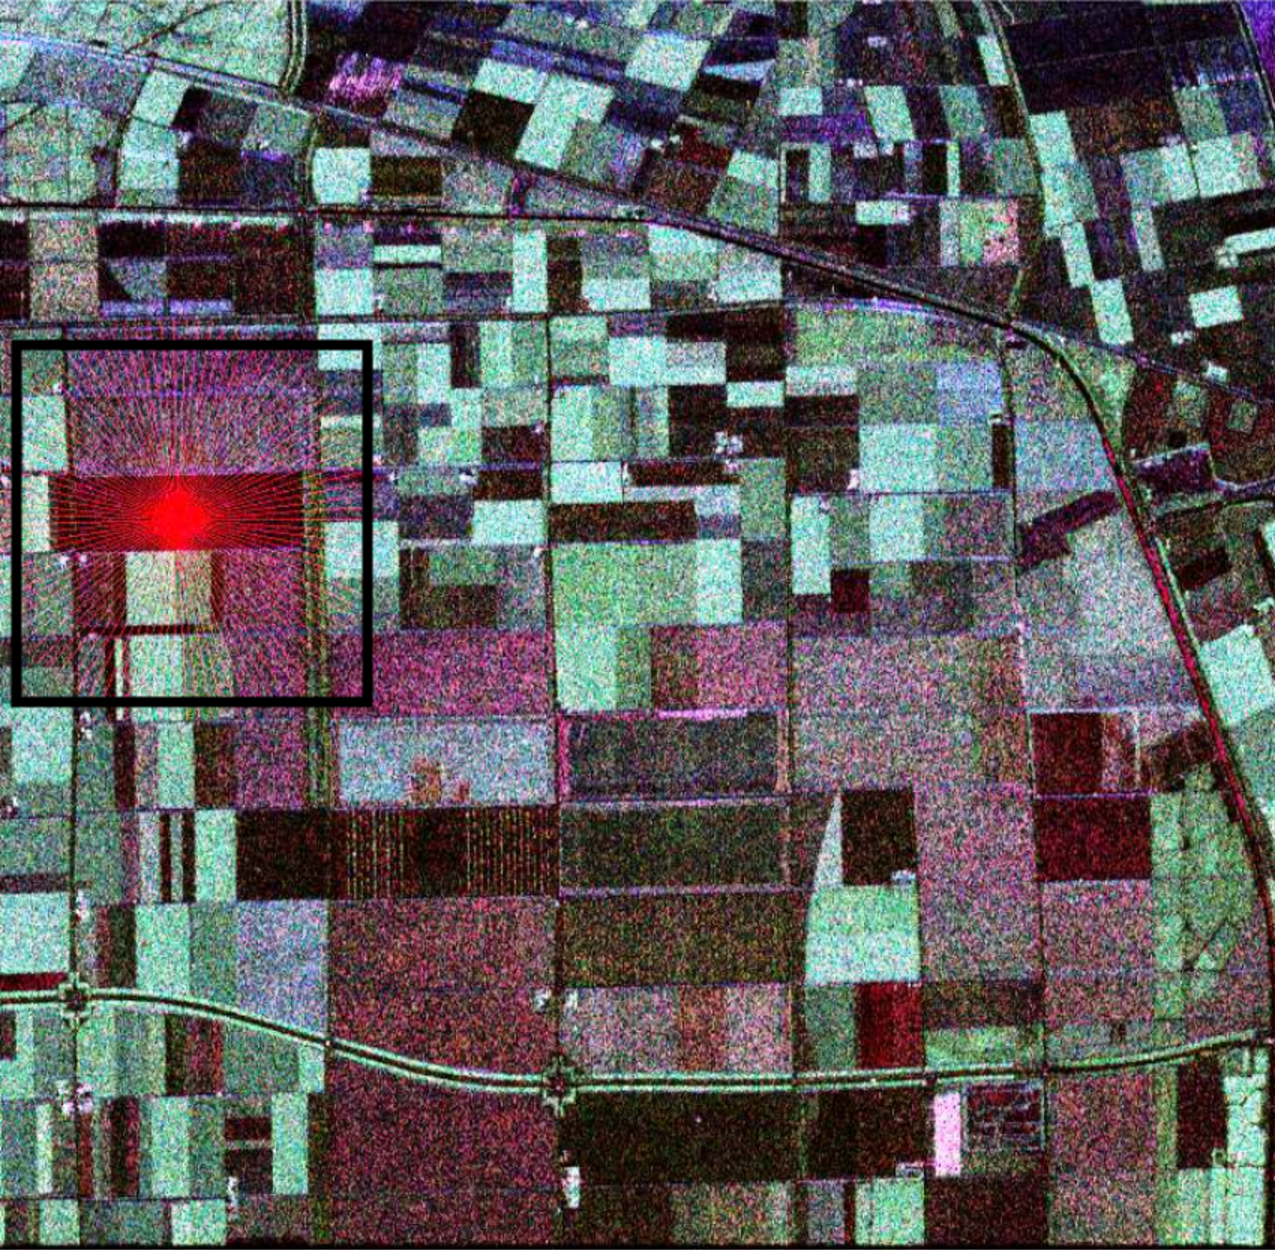
\includegraphics[width=.5\linewidth]{flevoland_radial_4_look_black}
	\caption{Region of interest (ROI) in the image of Flevoland.}
\label{flevoland_radial_4look}
\end{figure}
\end{alertblock}
\end{frame}


\begin{frame}[fragile]{PolSAR Image}
\begin{alertblock}{Numerical results}
	\begin{figure}[hbt]
	\centering
     \subfloat[Evidences in channel $\text{hh}$ \label{evidencias_hh_hv_vv:a}]{%
     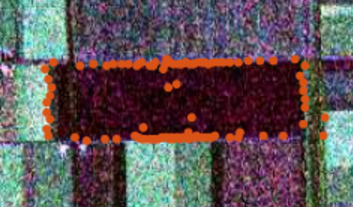
\includegraphics[width=0.3\textwidth]{flevoland_100_point_hh_crop}              
      % 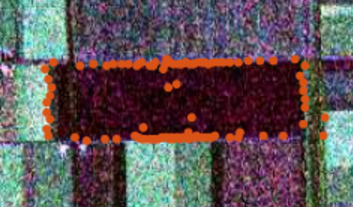
\includegraphics[viewport= 100 0 490 460, clip=true, width=0.3\linewidth]               {flevoland_100_point_hh_crop}
     }\qquad
     \subfloat[Evidences in channel $\text{hv}$ \label{evidencias_hh_hv_vv:b}]{%
       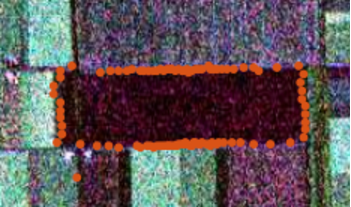
\includegraphics[width=0.3\linewidth]{flevoland_100_point_hv_crop}
     }\qquad
     \subfloat[Evidences in channel $\text{vv}$ \label{evidencias_hh_hv_vv:c}]{%
       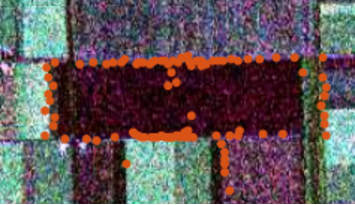
\includegraphics[width=0.3\linewidth]{flevoland_100_point_vv_crop}
     }
%     \caption{Edges evidences}
     \label{evidencias_hh_hv_vv}
   \end{figure}	
\end{alertblock}
\end{frame}

\begin{frame}[fragile]{PolSAR Image}
\begin{alertblock}{Numerical results}
	\begin{figure}[hbt]
	\centering
     \subfloat[Average Fusion \label{evidencias_hh_hv_vv:a}]{%
       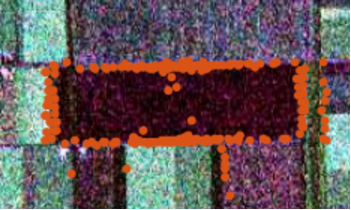
\includegraphics[width=0.3\linewidth]{flevoland_100_media_crop}
     }\quad
     \subfloat[PCA Fusion\label{evidencias_hh_hv_vv:b}]{%
       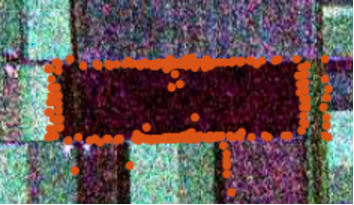
\includegraphics[width=0.3\linewidth]{flevoland_100_pca_crop}
     }\\
     \subfloat[SWT Fusion \label{evidencias_hh_hv_vv:a}]{%
       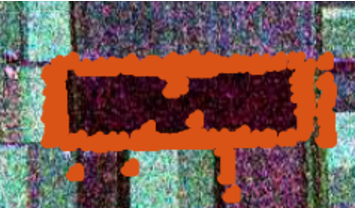
\includegraphics[width=0.3\linewidth]{flevoland_100_swt_crop}
     }\quad
     \subfloat[ROC Fusion \label{evidencias_hh_hv_vv:c}]{%
       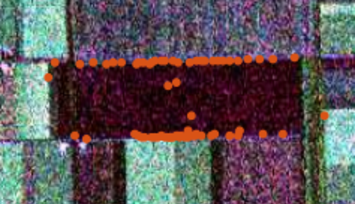
\includegraphics[width=0.3\linewidth]{flevoland_100_roc_crop}
     }
%     \caption{Edges evidences}
     \label{evidencias_hh_hv_vv}
   \end{figure}	
\end{alertblock}
\end{frame}

\begin{frame}[fragile]{PolSAR Image}
\begin{alertblock}{Conclusion}
\begin{itemize}
	\item Simulated Annealing works very well;
	\item The method to compute edges evidence in each channel works very well;
	\item Increase the number of channels to improve the fusion;
	\item Investigate new fusion methods.
\end{itemize}
\end{alertblock}
\end{frame}

\begin{frame}[allowframebreaks]
\bibliographystyle{IEEEtran}
\bibliography{../bibliografia}
\end{frame}

\end{document}
